% -----------------------------------------------
% Template for ISMIR Papers
% 2025 version, based on previous ISMIR templates

% Requirements :
% * 6+n page length maximum
% * 10MB maximum file size
% * Copyright note must appear in the bottom left corner of first page
% * Clearer statement about citing own work in anonymized submission
% (see conference website for additional details)
% -----------------------------------------------

\documentclass{article}
\usepackage[T1]{fontenc}
\usepackage[utf8]{inputenc}
\usepackage{ismir} % Remove the "submission" option for camera-ready version
\usepackage{amsmath,cite,url}
\usepackage{graphicx}
\usepackage{color}

\usepackage{amssymb}
\usepackage{bbm}
\usepackage{booktabs}

\newcommand{\dif}{\mathop{}\!\mathrm{d}}


\title{Collection of Notes for Boundaries and Labels}

% ---------------
\oneauthor
  {Qingyang (Tom) Xi}
  {NYU MARL\\\texttt{tom.xi@nyu.edu}}


\def\authorname{Q. Xi}
\sloppy % please retain sloppy command for improved formatting

\begin{document}

\maketitle

\begin{abstract}
Conceiving the segmentation task without unnecessary sampling.
Let's lose the frames.

\end{abstract}

%!TEX root = ../main.tex
%!TEX encoding = UTF-8
%!TEX spellcheck = en_US
%!TEX program = pdflatex

\section{Planning Ground}
Let's figure out what the plan is here:

\begin{description}
    \item[Flat Metrics] 
        Write it up.
        We did some writing for triplet based metrics, let's do the same for flat metrics.
    \item[Implementation] 
        Let's implement what's written in the test suites.
        We need to test their results and run speed.
\end{description}
% !TeX root = ../main.tex
% !TeX encoding = UTF-8
% !TeX spellcheck = en_US
% !TeX program = pdflatex

\section{Evaluating Flat Segmentations}
\subsection{Pairwise Clustering}
For evaluating how the segments are labeled, metrics are inspired by casting the segmentation problem as a clustering problem, where different atomic structural units (audio frame, beat, or measure) are clustered according to their segment labels.
Pairwise Frame Clustering (PFC) score is such an adaptation: it uses the same concept of precision and recall as above, but focusing on whether pairs of frames are labeled consistently~\cite{levy2008structural}.

Using $L: t \rightarrow \{y_1, \ldots, y_k\}$ to denote the reference label at time $t$, the set of time point pairs $\rho = \{(u, v)|L(u)=L(v)\}$ is defined as all $u, v$ pairs that are labeled identically by $L$.

Pairwise frame clustering metrics are then defined as follows: 
\begin{align*}
\text{PFC}_R = \frac{|\rho_\text{ref} \cap \rho_\text{est}|}{|\rho_\text{ref}|}&, \quad
\text{PFC}_P = \frac{|\rho_\text{ref} \cap \rho_\text{est}|}{|\rho_\text{est}|} \\
\text{PFC}_F = &\frac{2}{\frac1{\text{PFC}_R} + \frac1{\text{PFC}_P}}
\end{align*}
We can visualize the labels of a segmentation by plotting its Annotation Agreement Map (AAM) $A(u, v) = [(u, v) \in \rho]_\mathbbm{1}$ as is done in figure~\ref{fig:flat_anno_meet}.
Notice $|\rho|$ represents the number of non zero entries in $A(u, v)$, and $|\rho_\text{ref} \cap \rho_\text{est}|$ represent the number of pairs in the overlapping areas between $A_\text{ref}(u, v)$ and $A_\text{est}(u, v)$.

% \begin{figure}
%     \centering
%     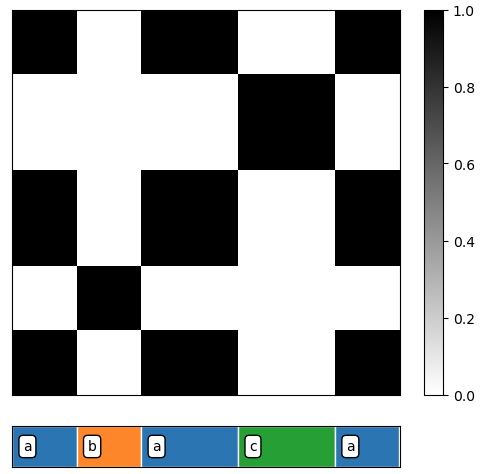
\includegraphics[width=0.5\linewidth]{content/figs/flat_anno_meet.png}
%     \caption{Annotation Agreement Map for the simple Rondo structure represented at the bottom}
%     \label{fig:flat_anno_meet}
% \end{figure}

\subsection{V-measure}
Inherent from its definition, the PFC metric favors coarser segmentations where its $A_\text{est}(u, v) = 1$ for large ranges of $u$ and $v$.
This incentivized the adoption of V-measure, another clustering metric, which is the current standard for comparing flat segmentations' labels~\cite{lukashevich2008towards}.
Instead of simply counting occurrences, V-measure looks at the normalized entropy of the true labels conditioned on their estimated label, and vice versa.
For a labeled segmentation $L(t)$ using a set of $k$ labels $\gamma = \{y_1, \ldots, y_k\}$, the entropy of the label distribution can be examined by sampling randomly along its duration:
$$\mathbb{H}(L(t)) = \underset{{y\in\gamma}}{\mathbb{E}}[-\log\mathbb{P}(L(t) = y)]$$
$\mathbb{H}(L(t))$ measures the uncertainty in the distribution defined by $\mathbb{P}(L(t))$ and equals to 0 when the distribution is deterministic (i.e. $L(t) = y_1$ for all $t$). 

$$\mathbb{H}(L_\text{ref} | L_\text{est}) = \underset{y\in\gamma}{\mathbb{E}}[\mathbb{H}(L_\text{ref} | L_\text{est}(t) = y)]$$
is the conditional entropy, which looks at the entropy of reference frame labels only when they receive the same label in the estimate segmentation.
Conceptually, the conditional entropy estimates the amount of uncertainty left in predicting the reference labels given the estimate segmentation.
When the uncertainty for reference label is low given the estimated label, the estimate recalls the labeling information presented in the reference.

V-measure normalizes the conditional entropy by the marginal entropy of the segment labels to calibrate scores for segmentations that have different number of distinct labels.
\begin{align*}
\text{V}_R = 1 - \frac{\mathbb{H}(L_\text{ref} | L_\text{est})}{\mathbb{H}(L_\text{ref})}&, \quad
\text{V}_P = 1 - \frac{\mathbb{H}(L_\text{est} | L_\text{ref})}{\mathbb{H}(L_\text{est})} \\
\text{V}_F = &\frac{2}{\frac1{\text{V}_R} + \frac1{\text{V}_P}}
\end{align*}

%!TEX root = ../main.tex
%!TEX encoding = UTF-8
%!TEX spellcheck = en_US
%!TEX program = pdflatex

\section{Triplet-based Metrics}\label{sec:hierarchy_metrics}
Two established MSA metrics for comparing hierarchies exist: the T-measure~\cite{DBLP:conf/ismir/McFeeNB15} which compares two sets of hierarchical boundaries, and the L-measure~\cite{McfeeNFB17} which also accounts for segment labeling.
Both metrics are implemented in \texttt{mir\_eval}~\cite{DBLP:conf/ismir/RaffelMHSNLE14} and have been used in many recent works on hierarchical MSA~\cite{DBLP:journals/taslp/BuissonMEC24, DBLP:conf/icassp/TralieM19, DBLP:journals/tismir/BerardinisVCC20, DBLP:conf/apsipa/ChenSY23}.

In this section, we provide a unifying overview for both measures, as they share the same core idea of recalling sets of triplets of time points $(t,u,v)$.
We begin by showing how L-measure and different variations of the T-measure can be thought of as specialized forms of L-measure.
% We do this in the hope that it will provide a better understanding of how the metrics work and better intuition about interpreting their results.

\subsection{Discrete set formulation}
We begin by laying down the notational framework by following prior literature~\cite{DBLP:journals/tismir/NietoMWSSGM20,DBLP:journals/tismir/KinnairdM21}.

For a piece of music with time span \(T = [t_0, t_1]\), a flat segmentation has a label mapping $S(t)$:
\begin{equation}
    S(t): T \to \{y_1, y_2, \ldots\}.
    \label{eq:S}
\end{equation}
A $k$-level hierarchy is then a sequence of progressively finer segmentations
\(H = \bigl(S_{1}, S_{2}, \dots, S_k\bigr)\).

Given a hierarchy $H$, L-measure defines a relevance mapping $M$ between time point pairs $T \times T$ as the maximum level of the hierarchy at which the two time points share the same label:
\begin{equation}
    M_H(u, v) := \max \big\{k \, | \, S_k(u) = S_k(v)\big\}
    \label{eq:relevance_mapping}
\end{equation}
This is called the meet matrix of two hierarchical annotations in prior literature.

% Let's visualize some of these concepts. Show hierarchy H, M(u, v|H), and the orientation map $I_H(t,u,v)$ at a given time $t$.

Triplet based metrics are interested in the set \(\mathcal{A}(H)\) consisting of time-triplets \((t,u,v)\) where the time instances $t$ and $u$ are deemed more relevant than $t$ and $v$.
L-measure defines its significant set of triplets as:
\begin{equation}
    \mathcal{A}(H) = \{(t,u,v)|M_H(t,u) > M_H(t,v)\}
\end{equation}

Precision and recall scores are then defined by counting the proportions of triplets shared between the derived sets.
For an estimated hierarchy $\hat{H}$ and a reference $H$, we define:
\begin{align}
\mathrm{L}_{\mathrm{recall}}(\hat{H} \mid H )
&= \frac{\bigl|\mathcal{A}(\hat{H}) \,\cap\, \mathcal{A}(H)\bigr|}
    {\bigl|\mathcal{A}(H)\bigr|}, \nonumber \\
\mathrm{L}_{\mathrm{precision}}(\hat{H} \mid H ) \label{eq:lmeasure}
&= \frac{\bigl|\mathcal{A}(\hat{H}) \,\cap\, \mathcal{A}(H)\bigr|}
    {\bigl|\mathcal{A}(\hat{H})\bigr|}.
\end{align}

In the discrete set formulation, $|\mathcal{A}(H)|$ is the cardinality of a set of triplets. 
This necessitates a frame-based sampling of time triplets for metric calculation, which is computationally expensive for long sequences.
Furthermore, this sampling-based approach is an approximation that depends on time resolution, which by convention is set to 0.1 seconds.

 
\subsection{Continuous set Formulation}
We can also define the triplet recall metric in continuous time.
The set-based definition of hierarchy metrics could be expressed in terms of areas or volumes in space, which allows us to avoid the frame-based sampling of triplets.
Because $S_k(t)$ is piecewise constant, the integrals involved can all be computed in closed form, with complexity related to the number of segments in the hierarchy rather than the number of frames.

Triplet-based metrics differ only in how they define the pair relevance mapping \(M_H(u,v)\) and the significant triplet indicator \(I_H(t,u,v)\), which for L-measure is defined as:
\begin{equation}
    I_H(t,u,v) = \big[M_H(t,u) > M_H(t,v)\big]_{\mathbbm{1}}, 
    \label{eq:significant_triplet}
\end{equation}
where \([\,\cdot\,]_{\mathbbm{1}}\) is the indicator function that returns 1 if the condition is true and 0 otherwise.

Using the significant triplet indicator $I_H(t,u,v)$, we can calculate the structural richness at time $t\in T$ as a measure.
\emph{Structural information measure} is defined for each time point $t$ as:
\begin{equation}
    \iota(H;t) = \int_{T^2} I_H(t,u,v)\,\dif(u,v).
    \label{eq:local_richness}
\end{equation}
This measure captures the amount of structural information present at time \(t\) in the hierarchy \(H\).

As opposed to integrating over the $(t,u,v) \in T \times T \times T$ directly, we first integrate over the time pairs \((u,v) \in T \times T\) to obtain measures at \(t\), before aggregating over $t \in T$, as is done in the original implementation of the metric.
Doing this would mean each time point \(t\) contributes equally to the overall measure, irrespective of the amount of structural information at $t$.

We call the intersection of information between the two hierarchies \(H\) and \(\hat{H}\) the \emph{structural agreement measure} at time \(t\):
\begin{equation}
    \alpha_H(\hat{H};t) = \int_{T^2} I_H(t,u,v)\cdot I_{\hat{H}}(t,u,v)\,\dif(u,v).
    \label{eq:local_agreement}
\end{equation}

The ratio between these two measures then gives us the portion of structural information at time $t$ on a reference hierarchy \(H\) is being recalled.
We call $\rho_H$ the local recall density of $\hat{H}$ on $H$:
\begin{equation}
    \rho_H(\hat{H};t) = \frac{\alpha_H(\hat{H};t)}{\iota(H;t)}.
    \label{eq:local_recall}
\end{equation}

Finally, we can define the overall recall as the average local recall density over time.
Notice that $\rho_H(\hat{H};t)$ is only defined for times where there is any information to recall at time $t$.
We define this informative subset of time span as 
\[
    \mathcal{T}_H = \{t \in T | \iota(H;t) > 0\}.
\]

This leads to the definition of L-measure:
\begin{align}
    \mathrm{L}_{\mathrm{recall}}(\hat{H} \mid H) 
    &= \frac{1}{|\mathcal{T}_H|}
    \int_{\mathcal{T}_H} \rho_H(\hat{H};t)\, \dif t, \nonumber \\
    \mathrm{L}_{\mathrm{precision}}(\hat{H} \mid H) 
    &= \frac{1}{|\mathcal{T}_{\hat{H}}|}
    \int_{\mathcal{T}_{\hat{H}}} \rho_{\hat{H}}(H;t)\, \dif t,
    \label{eq:new_lmeasure}
\end{align}
where \(|\mathcal{T}_H| = \int_{\mathcal{T}_H} \dif t\) is the total duration of informative time spans under $H$.

\subsection{Variations}
By using alternative definitions for time pair relevance induced by the hierarchy \(M\) and the significant triplet selection criteria \(I\), we can formulate the T-measure and its different variations.

\subsubsection{Full T-measure}
As mentioned, the T-measure can be seen as a variation of the L-measure, where the relevance mapping disregards label information.
If we label each segment in the hierarchy with a unique label, the full T-measure without windowing is equivalent to the L-measure.

In other words, we can express T-measure's relevance mapping as:
\begin{equation}
    M_H(t,u) = \max \big\{
        k \, | \, S^*_k(t) = S^*_k(u)
    \big\},
    \label{eq:tmeasure_relevance_map}
\end{equation}
where $S^*_k(t)$ identifies the segment containing $t$ at level $k$, as opposed to $S_k(t)$ which gives the label at time $t$.

\subsubsection{Reduced T-measure}
The reduced T-measure differs from the full T-measure by using an alternative definition for significant triplet indicator.
For reduced T-measure, the significant triplet are those where $u$, and $v$'s relevance to $t$ differ by exactly one level:
\begin{align}
    I'_H(t,u,v) = \big[ M_H(t,u) - M_H(t,v) = 1\big]_{\mathbbm{1}}.
    \label{eq:reduced_tmeasure}
\end{align}
This means that the reduced T-measure is only sensitive to refinements between consecutive levels of the hierarchy, as opposed to the overall ranking of all levels.

\subsubsection{Windowed T-measure}
The windowed T-measure extends the definition of $\iota_H(t)$ for using a time-varying window $W(t)$ around $t$ as the integration range, as opposed to integrating directly over the full time span.

Let $W(t) = \big( [t - w, t + w] \cap T\big)$ be a sliding window of size $\leq 2w$ around $t$.
We define the windowed structural information measure by changing the range of integration from the original:
\[
    \iota^W(H;t) = \int_{W^2(t)} I_H(t,u,v)\,\dif(u,v), 
    \label{eq:windowed_richness}
\]
\[ \displaystyle
    \alpha^W_H(\hat{H};t) = \int_{W^2(t)} I_H(t,u,v)\cdot I_{\hat{H}}(t,u,v)\,\dif(u,v) 
    \label{eq:windowed_agreement}
\]


The rest of the definitions follow.

\subsubsection{Monotonicity and the concept of relevance}
The relevance mapping \(M_H(u,v)\) for triplet-based metrics shown in ~\eqref{eq:relevance_mapping} assumes that H has monotonic labeling.
However, in practice, label monotonicity is often violated, and the current definition of \(M_H(u,v)\) can give rise to counterintuitive results.

Alternatively, we can formulate the relevance mapping with requirement for strict label monotonicity:
\begin{equation}
    M'_H(u,v) = \min \bigl\{k \, |\, S_i(u) \neq S_i(v)\bigr\} - 1,
    \label{eq:monotonic_meet}
\end{equation}
which measures the deepest level that two time points meet monotonicly by first finding the shallowest level where the two time points diverge in labeling.

Notice how for a monotonic hierarchy $H$, the two versions of the relevance mapping are equivalent: $M'_H(u,v) = M_H(u,v)$.  

In case where the hierarchy is not monotonic, the two definitions of relevance mapping can lead to different results.
Put in FIGURE that shows how M and M' for a non-monotnoic hierarchy.
While monotonicity is not a requirement for the triplet based metrics, we will see how using this substitute definition of relevance mapping can lead to different results when monotonicity is violated.


\bibliography{content/refs}
\end{document}
